\documentclass[review,12pt]{elsarticle}
\usepackage{amsmath,amssymb}
\usepackage{booktabs,tabularx,array,longtable}
\usepackage{graphicx,float,pdflscape}
\usepackage{siunitx}
\usepackage{url,hyperref}
\usepackage[T1]{fontenc}
\usepackage[utf8]{inputenc}
\setlength{\emergencystretch}{3em}
\journal{Applied Energy}
\begin{document}
\begin{frontmatter}
\title{OpenDC-LCA: boundary-aware evidence synthesis for data-center cooling under grid decarbonization}
\author[uark]{Han Hu\corref{cor1}}
\author[uark]{Darin W. Nutter}
\address[uark]{Department of Mechanical Engineering, University of Arkansas, Fayetteville, Arkansas, USA}
\cortext[cor1]{Corresponding author}
\begin{abstract}
Life-cycle assessments (LCAs) of data-center cooling often report rankings despite differences in electricity accounting, useful-computation equivalence, boundaries, and foreground data. OpenDC-LCA links cooling engineering and LCA tools. We reconciled 24 released totals from a Microsoft/WSP study, reconstructed nine U.S. EPA eGRID years on a common AR5 GWP100 basis, and tested anchor coverage, boundary mismatch, functional-unit equivalence, assumption blocks, dependence, and numerical convergence. The harmonized U.S. generation rate declined 32.46\%, from 517.73 kg CO2e/MWh in 2012 to 349.67 kg CO2e/MWh in 2023; GWP-basis harmonization changed any annual national rate by at most 0.248 kg CO2e/MWh. Yet 137 of 459 state-year rates lay outside the released electricity anchors. The cold-plate/single-phase crossover was 96.7 kg CO2e/MWh. The only 2023 state below it lost that ordering after an exact 73.01 kg CO2e/MWh additive boundary test. Two-phase immersion ranked first in every deterministic state-year screen, but its U.S. first-rank frequency fell from 99.19\% to 55.05\% across narrow-to-wide all-block zero-correlation stress designs. In the wide design it rose from 55.05\% with independent architecture errors to 100\% with common-mode errors; embodied variation caused the largest one-block rank loss. A median 5.50\% adverse useful-computation correction also erased first rank. These frequencies describe stress designs, not probabilities. The national decarbonization trend is stable, whereas cooling rankings depend on boundary, foreground, dependence, and service-equivalence evidence. OpenDC-LCA converts those dependencies into traceable data requirements rather than a universal league table.

\end{abstract}
\begin{keyword}
data center \sep life-cycle assessment \sep immersion cooling \sep grid
\end{keyword}
\end{frontmatter}

decarbonization; uncertainty; functional unit; open-source software

\section{Introduction}
\subsection{Cooling is an energy-system and lifecycle decision}
Data centers couple rapidly changing computing hardware to long-lived buildings, electrical systems, cooling plants, and regional energy and water systems. Global data-center electricity estimates remain uncertain, but the scale and growth of cloud and artificial-intelligence workloads make energy efficiency and supply decarbonization simultaneous design constraints \cite{ref1,ref2}. At the equipment level, increasing processor heat flux and rack density are driving a transition from room air cooling toward rear-door heat exchangers, direct-to-chip cold plates, and single- or two-phase immersion \cite{ref3,ref4,ref5}.

These alternatives are not interchangeable heat exchangers. They alter server fans, pumps, coolant distribution units, heat-rejection temperature, fluid inventory, rack or tank construction, packing density, repair procedures, and sometimes achievable clock rate. System experiments have reported materially different coefficient of performance and cost behavior for single- and two-phase immersion over load \cite{ref6}, while recent single-phase tests show that flow direction, coolant viscosity, and water temperature affect chip temperature, thermal resistance, and PUE \cite{ref7}. Two-phase experiments similarly show that boiling, pressure stability, and condenser performance must be evaluated at server and system levels \cite{ref8}. A comparison at equal rack count, equal IT electricity, or equal nameplate capacity can therefore compare different computational services.

PUE remains useful for facility energy management, but it is not a lifecycle functional unit and does not represent hardware production, cooling-fluid loss, replacement, water scarcity, or useful computation. Cooling selection is therefore an energy-system decision with lifecycle consequences, not a single-metric efficiency contest.

\subsection{What existing data-center LCAs show}
Early environmental assessments showed that operating electricity dominates many data-center footprints and that PUE alone can transfer burdens outside the measured facility boundary \cite{ref9}. U.S. studies subsequently linked data centers to spatially varying electricity and water burdens \cite{ref10,ref11}. At the product scale, Isler-Kaya and Karaosmanoglu collected manufacturing inventory for a cooling device and evaluated electricity and waste scenarios \cite{ref12}. Wenzel and Radgen compared energy, material-flow, exergy, and lifecycle assessment methods for a wet cooling tower, illustrating that method choice changes the question answered \cite{ref13}.

Alissa et al. published the most detailed public hyperscale comparison of air, cold-plate, single-phase immersion, and two-phase immersion \cite{ref14}. Their cradle-to-grave model included buildings, support equipment, servers, racks or tanks, cables, cooling fluids, use-phase electricity and water, replacement, and end of life. The use of Vcore-year as the functional unit was a major advance because it allowed packing density and cooling-enabled computation to enter the comparison. The accompanying archive includes normalized contributions, equations, uncertainty material, and a pedigree assessment \cite{ref15}. It does not, however, disclose every licensed background process, architecture-specific bill of quantities, or a transferable mapping from electricity to workload performance.

Recent LCA work confirms that electricity decarbonization and cooling efficiency are complementary but can shift impacts among categories \cite{ref16}. Manufacturer and ICT studies also show wide dispersion in embodied server impacts \cite{ref17,ref18}. Together, these studies show the need for lifecycle assessment while exposing a transferability problem: a static result at one grid, one performance assumption, and one database system cannot be treated as a universal cooling ranking.

\subsection{Electricity accounting, time, and geography}
Electricity is not a scalar independent of method. Attributional LCA usually requires a consumption mix with upstream generation, transmission, and other indirect processes, whereas eGRID state total-output rates describe direct emissions from in-state generation. Location-based, market-based, and marginal factors answer different questions. Combining location- and market-based accounting inconsistently can double count renewable attributes \cite{ref19,ref20}. Average rates can also fail to represent the effect of workload shifting; Dandres et al. found that average and marginal electricity signals can lead to different real-time data-center decisions \cite{ref21}.

Time enters at several levels: cooling performance varies with load and weather; grid composition varies hourly and over years; equipment is replaced at discrete times; and background technologies evolve. Dynamic-LCA reviews distinguish temporal inventory, characterization, and prospective background change \cite{ref22,ref23}. Open tools such as Temporalis and, more recently, bw\_timex show how temporal information can be propagated through process networks \cite{ref24,ref25,ref26}. For cooling, hourly operation is necessary but insufficient: the grid method, geography, and upstream boundary must also be aligned. A weather file cannot repair an incompatible electricity inventory.

\subsection{Data quality, uncertainty, and the decision value of evidence}
LCA uncertainty arises from parameters, scenarios, model form, allocation, system boundary, and incomplete knowledge. Monte Carlo propagation is useful when distributions and correlations are supportable; it becomes misleading when arbitrary ranges are presented as confidence. Reviews recommend separating variability from uncertainty and using sensitivity analysis to identify influential assumptions \cite{ref27}. Pedigree matrices can communicate reliability, temporal, geographic, and technological representativeness, but the conversion from qualitative scores to uncertainty is itself a modeling choice \cite{ref28,ref29}.

Data-quality assessment is therefore not a decorative appendix. EPA guidance emphasizes reproducible documentation at flow and process levels \cite{ref29}. Decision analysis goes further: value-of-information methods prioritize data whose resolution is expected to change a decision, rather than simply improving every weak input \cite{ref30}. This distinction is important for electronics-cooling laboratories. A parameter may have poor pedigree but negligible decision leverage; a seemingly precise PUE difference may be decisive if two lifecycle alternatives are nearly tied.

The review standard also depends on the claim. ISO 14040 and ISO 14044 define the LCA framework and requirements, whereas ISO 14071:2024 specifies critical review processes and reviewer competencies, with particular relevance to comparative assertions intended for public disclosure \cite{ref31,ref32}. Code tests, data checks, and coauthor review can strengthen traceability, but none is a substitute for an independent critical review.

\subsection{Research gap and contribution}
General engines such as openLCA and Brightway calculate process networks, exchange inventories, and apply LCIA methods \cite{ref33,ref34}. They do not determine whether cooling alternatives deliver equivalent computation, whether a performance map covers the operating domain, whether a grid substitution preserves the original electricity boundary, or whether secondary screening results support a public comparative assertion.

Five gaps remain at the intersection of cooling engineering and LCA:

\begin{enumerate}
\item published normalized totals cannot be transparently updated when foreground
quantities and licensed process mappings are incomplete;

\item annual, static results hide grid, weather, and load transferability;
\item common-unit electricity factors can retain incompatible characterization
methods and system boundaries;

\item qualitative data-quality scores do not directly show which measurement
could change the technology decision; and

\item software often produces a number without preserving whether it is
reconstructed, screened, empirically supported, or suitable for a comparative claim.

\end{enumerate}

This study addresses those gaps with a boundary-aware evidence layer and a secondary analysis of the released Microsoft/WSP case. The specific contributions are:

\begin{enumerate}
\item exact arithmetic reconstruction of 24 released architecture-scenario-impact
totals;

\item a common-basis reconstruction of nine eGRID releases from gas-specific
emissions rather than comparison of provider CO2e fields with changing GWP conventions;

\item explicit diagnostics for anchor extrapolation, electricity-boundary
mismatch, useful-computation equivalence, and joint assumption stress;

\item transparent use of Boavizta, ÖKOBAUDAT, USLCI, GLAD, NOAA, and USGS data
according to their supported numerical role; and

\item an open package that emits both results and an evidence/claim classification.
\end{enumerate}

The aim is not to independently reproduce a proprietary product system or declare a winning cooling technology. It is to determine which conclusions survive disclosed transformations and which require new measurements.

\section{Framework and methods}
\subsection{Evidence-to-decision architecture}
Figure 1 shows the OpenDC-LCA workflow. Every source is registered with provider, version, persistent identifier or URL, geography, reference year, declared unit, boundary, license or redistribution constraint, evidence class, and checksum. The harmonization stage then asks, in order: are the alternatives functionally equivalent; are the units, characterization methods, time, and geography aligned; is the required transformation interpolation or extrapolation; and are uncertainty, correlation, and review status adequate for the proposed claim? The result is classified as reconstructed, screening-transformed, registered/unlinked, or supported by primary decision-grade evidence.

\begin{figure}[!htbp]
\centering
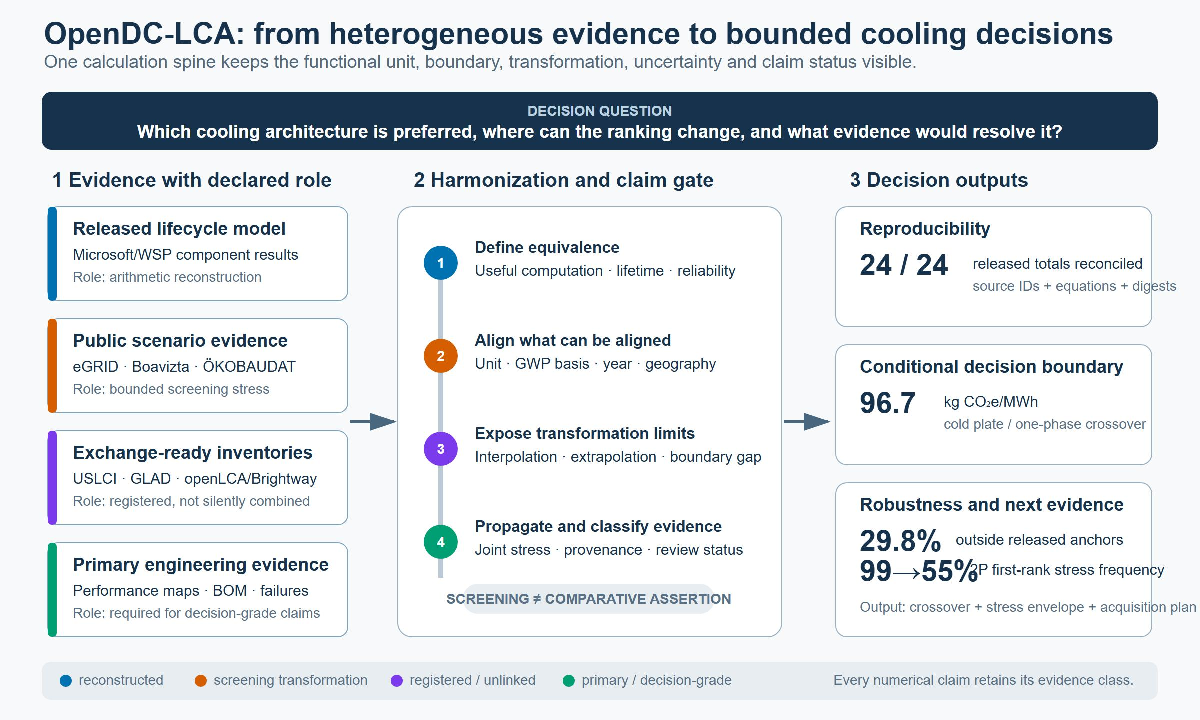
\includegraphics[width=0.98\linewidth]{figures/figure0_opendc_lca_workflow.pdf}
\caption{OpenDC-LCA evidence-to-decision architecture. Inputs are assigned a numerical role before calculation. The harmonization spine makes functional equivalence, method alignment, extrapolation, uncertainty, and claim status explicit. Outputs combine the numerical result with its evidence class and next-data requirement.}
\label{fig:figure0-opendc-lca-workflow}
\end{figure}

OpenDC-LCA is implemented in Python 3.10 or later and distributed under the MIT License \cite{ref35}. Version 1.1.0 provides a command-line interface, Python API, local browser GUI, scenario and performance-map schemas, reliability and replacement models, openLCA JSON-LD and Brightway mappings, evidence audits, and human- and machine-readable reports. All interfaces call the same calculation engine.

\subsection{Goal, functional units, and system boundaries}
The practitioner package defaults to one MWh delivered to IT equipment (\texttt{it\_mwh}) for operational screening. That unit is valid for comparison only when alternatives provide equivalent computational output, utilization, quality of service, reliability, and hardware life. The Microsoft/WSP secondary analysis remains in its released functional unit of one Vcore-year. No conversion between IT MWh and Vcore-year was made because the public archive does not provide a workload-independent mapping between them.

The package supports a cooling-system cradle-to-grave boundary and a broader facility cradle-to-grave boundary. The former includes cooling and heat-rejection equipment, fluids, represented maintenance and replacement, operation, and end of life. The latter can also include building, electrical, and IT assets. Common systems may be excluded only when their quantity, performance, lifetime, and end-of-life treatment are unchanged. Onsite water and electricity-supply-chain water are reported separately; location- and market-based electricity are not merged.

\subsection{Dataset roles and inclusion logic}
Table 1 states how each downloaded source enters this study. This is an important methodological control: being readable by the software does not make a dataset compatible with the case model.

{\footnotesize
\setlength{\tabcolsep}{3pt}
\begin{longtable}{>{\raggedright\arraybackslash}p{0.18\textwidth}>{\raggedright\arraybackslash}p{0.23\textwidth}>{\raggedright\arraybackslash}p{0.34\textwidth}>{\raggedright\arraybackslash}p{0.16\textwidth}}
\caption{Numerical role and boundary assigned to downloaded evidence.}\\
\toprule
Source and evidence used & Numerical role in this paper & Boundary or transfer limit & Claim class \\
\midrule
\endfirsthead
\caption[]{Numerical role and boundary assigned to downloaded evidence. (continued)}\\
\toprule
Source and evidence used & Numerical role in this paper & Boundary or transfer limit & Claim class \\
\midrule
\endhead
\midrule
\multicolumn{4}{r}{Continued on next page}\\
\endfoot
\bottomrule
\endlastfoot
Microsoft/\allowbreak{}WSP archive: 24 totals, component tables, 2 electricity anchors, pedigree records \cite{ref14,ref15} & Arithmetic reconstruction, foreground contribution model, crossover and stress analyses & Licensed background inventories and complete bills of quantities are not public & Released/\allowbreak{}reconstructed \\
\addlinespace[2pt]
EPA eGRID: 459 state/\allowbreak{}DC-\allowbreak{}year rows and 9 U.S. aggregates \cite{ref36,ref37} & Common-\allowbreak{}basis generation-\allowbreak{}rate scenarios and historical trend & Direct generation rates are not consumption-\allowbreak{}based lifecycle electricity inventories & Screening transformation \\
\addlinespace[2pt]
Boavizta: 48 server PCF records \cite{ref38} & Server-\allowbreak{}manufacturing dispersion and common-\allowbreak{}scaling stress & Products, configurations, PCRs, lifetimes, and performance are heterogeneous & Secondary cross-\allowbreak{}product evidence \\
\addlinespace[2pt]
ÖKOBAUDAT: 6 selected A1-\allowbreak{}A3 processes \cite{ref39} & Matched steel-\allowbreak{} and cement-\allowbreak{}route procurement levers & German generic factors require architecture-\allowbreak{}specific bills of quantities & Secondary process evidence \\
\addlinespace[2pt]
NOAA TMY: 8,760 Fayetteville weather rows \cite{ref40} & Performance-\allowbreak{}map and hourly-\allowbreak{}integration software test & No measured four-\allowbreak{}architecture cooling surface is available & Illustrative only \\
\addlinespace[2pt]
USLCI and 7 GLAD hydrogen archives \cite{ref41,ref42} & Exchange and interoperability tests & Product-\allowbreak{}system links, allocation, providers, and LCIA methods are unresolved & Registered/\allowbreak{}unlinked \\
\addlinespace[2pt]
USGS watershed boundary: HU12 geometry \cite{ref43} & Spatial data contract test & Geometry is not withdrawal, consumption, or water-\allowbreak{}scarcity characterization & Registered/\allowbreak{}unlinked \\
\addlinespace[2pt]
\end{longtable}
}

Provider-native raw files remain outside the public repository when redistribution permission is unclear. Derived tables retain filenames, worksheets, fields, units, and checksums.

\subsection{Static energy, equipment, fluid, and replacement calculations}
For IT capacity $P_\mathrm{IT}$, utilization $u$, and one year, annual IT electricity is

\[
E_\mathrm{IT}=P_\mathrm{IT}u(8760).
\tag{1}
\]

Facility electricity is

\[
E_\mathrm{facility}=E_\mathrm{IT}\mathrm{PUE}.
\tag{2}
\]

For operational impact factor $EF_k$, the operational impact per delivered IT electricity is

\[
I_{k,\mathrm{op}}=EF_k\mathrm{PUE}.
\tag{3}
\]

Equipment production and end-of-life burdens are annualized with discrete replacement:

\[
I_{k,\mathrm{eq}} =
\sum_i
\frac{q_i\left\lceil L_s/L_i\right\rceil
\left(I_{k,i}^{\mathrm{prod}}+I_{k,i}^{\mathrm{EOL}}\right)}
{L_s},
\tag{4}
\]

where $q_i$ is quantity, $L_s$ the study period, and $L_i$ service life. The package also supports a linear screening option. For initial fluid mass $m_0$, facility life $L_f$, annual loss $m_\mathrm{loss}$, production factor $I_k^\mathrm{fluid}$, and direct global-warming factor $GWP_\mathrm{direct}$,

\[
m_\mathrm{prod,annual}=\frac{m_0}{L_f}+m_\mathrm{loss},
\tag{5}
\]

\[
I_{k,\mathrm{fluid}}=m_\mathrm{prod,annual}I_k^\mathrm{fluid},
\qquad
GHG_\mathrm{direct}=m_\mathrm{loss}GWP_\mathrm{direct}.
\tag{6}
\]

These equations are part of the software engine. The secondary Microsoft/WSP analysis uses the normalized component values released by the authors rather than inventing missing quantities.

\subsection{Released-model reconstruction and electricity-intensity index}
For each of four cooling architectures, two electricity cases, and three impact metrics, the released total was recomputed as the sum of use phase, building, compute server, storage server, networking server, rack or tank, cable, support equipment, and cooling-fluid contributions. This 24-cell test is an arithmetic-consistency audit. It does not validate confidential quantities, licensed LCA for Experts or ecoinvent processes, allocation, performance, or field operation.

The detailed archive identifies the electricity anchors as 524.893 kg CO2e/MWh for U.S. average electricity and 6.133 kg CO2e/MWh for U.S. average wind under IPCC AR5 GTP100 excluding biogenic carbon. We define a numerical intensity-position index

\[
z_s=\frac{g_s-g_R}{g_G-g_R},
\tag{7}
\]

where $g_G$ and $g_R$ are the released GaBi electricity anchors and $g_s$ is an external screening rate. The released impact for technology $j$ is then transferred as

\[
I_{j,s}=I_{j,R}+\left(I_{j,G}-I_{j,R}\right)z_s.
\tag{8}
\]

Equations (7)-(8) reproduce both released endpoints exactly. They are not a background-process substitution. The Microsoft anchors are lifecycle GTP100 results; eGRID rates are direct power-sector GWP100 results. Common units do not remove the characterization and upstream-boundary mismatch. We therefore refer to $g_s$ as a screening index, count all extrapolations, and perform a separate boundary-mismatch stress.

The crossover of technologies $a$ and $b$ follows from equality in Eq. (8):

\[
g^*=g_R+(g_G-g_R)
\frac{I_{b,R}-I_{a,R}}
{(I_{a,G}-I_{a,R})-(I_{b,G}-I_{b,R})}.
\tag{9}
\]

\subsection{Common-basis eGRID reconstruction}
EPA changed the GWP values used by eGRID: releases before 2018 used IPCC SAR, 2018-2022 used AR4, and 2023 used AR5 without climate-carbon feedback \cite{ref36,ref37}. To remove this avoidable discontinuity, every state and U.S. factor was reconstructed from net generation and gas-specific annual emissions:

\[
g_{y}^{\mathrm{AR5}}=
\frac{2000M_{\mathrm{CO2},y}
+28M_{\mathrm{CH4},y}
+265M_{\mathrm{N2O},y}}
{E_y}(0.45359237),
\tag{10}
\]

where CO2 is reported in short tons, CH4 and N2O in pounds, $E_y$ in MWh, and the final factor converts pounds to kilograms. The provider-published CO2e rate was retained as a comparison. The provider U.S. aggregate, rather than the 50-state-plus-DC reconstruction, was used for national results. Puerto Rico was excluded from the state/DC panel; the resulting scope coverage was reported for each year.

The eGRID factors describe in-state generation. They are not consumption mixes, marginal rates, hourly signals, contractual procurement, or LCIs with upstream fuel and infrastructure. No state-specific LCA is claimed.

\subsection{Extrapolation, boundary, and functional-unit diagnostics}
Each of the 459 state-year rates was classified as below, between, or above the two released electricity anchors. Equation (8) is interpolation only for the middle class.

Because an upstream lifecycle difference between eGRID and the GaBi anchors cannot be estimated from the released files, we did not assign a best value. Instead, we added transparent allowances of 0, 25, 50, 75, and 100 kg CO2e/MWh to every 2023 eGRID rate and recomputed architecture order. This is a boundary-mismatch stress, not an uncertainty distribution or estimate of upstream emissions. We also calculated the exact additive value that moves the lowest 2023 state rate to the cold-plate/single-phase crossover, (g\textasciicircum{}*-min(g\_s)).

Functional-unit sensitivity was evaluated separately. At each state-year, the minimum multiplicative increase in two-phase impact per equivalent useful computation required to equal the second-ranked architecture was

\[
\delta_{\mathrm{service}}=
\frac{\min_{j\ne 2P}I_j}{I_{2P}}-1.
\tag{11}
\]

This correction represents an unresolved combination of useful throughput, server count, quality of service, lifetime, and replacement. It is not a measured two-phase penalty.

\subsection{Assumption-block and dependence stress designs}
Deterministic break-even values do not propagate interacting assumptions. We therefore ran seeded, 20,000-iteration triangular stress designs for the 2023 U.S. generation factor and the lowest-carbon 2023 state. The headline design used one shared grid multiplier and independent technology-specific multipliers for use phase, embodied contribution, and impact per equivalent service. It is the all-block, zero-correlation member of the dependence analysis described below. Three declared envelopes were used (Table 2).

\begin{table}[!htbp]
\centering
\caption{Declared half-widths for joint assumption-stress ensembles.}
\small
\setlength{\tabcolsep}{3pt}
\begin{tabularx}{\textwidth}{>{\raggedright\arraybackslash}p{0.15\linewidth}>{\raggedright\arraybackslash}p{0.39\linewidth}>{\raggedright\arraybackslash}p{0.18\linewidth}>{\raggedright\arraybackslash}p{0.18\linewidth}}
\toprule
Envelope & Grid, use, and service half-\allowbreak{}width & Embodied half-\allowbreak{}width & Purpose \\
\midrule
Narrow & $\pm$2\% & $\pm$20\% & Numerical stability near released values \\
Screening & $\pm$5\% & $\pm$50\% & Intermediate declared stress; not a fitted range \\
Wide & $\pm$10\% & $\pm$100\% & Deliberately severe robustness test \\
\bottomrule
\end{tabularx}
\end{table}

The triangular mode was 1.0 and the base seed was 20250730. A stable hash of the context, envelope, active block, and dependence case generated a separate seed for every design, so output does not depend on loop order. We then repeated the stress with grid only, use phase only, embodied contribution only, service equivalence only, and all four blocks active. Technology-specific multipliers were coupled with a Gaussian copula at declared latent correlations of 0, 0.5, and 1 while retaining the same triangular marginals. These correlations are not measurements. Rank frequencies describe the declared designs; they are not posterior probabilities, confidence levels, or a substitute for empirical uncertainty distributions.

Numerical convergence was checked with nested 5,000-, 20,000-, and 80,000-draw runs using the same scenario seeds. The binomial Monte Carlo standard error is reported only as integration precision within each declared design. It is not a confidence interval for cooling performance or a remedy for unsupported input distributions.

\subsection{Server, construction, and data-priority analyses}
Boavizta records were filtered to \texttt{Datacenter/Server} products with total GHG, manufacturing share, and lifetime. Manufacturing GHG was calculated as total product GHG times manufacturing share and annualized by declared lifetime. The minimum, quartiles, median, and maximum annualized values were divided by the empirical median and used only as common multiplicative stresses on the released compute, storage, and networking contributions. This preserves a unitless scale test without treating different servers as functionally interchangeable.

Selected ÖKOBAUDAT A1-A3 steel and cement records were compared within product families:

\[
R=100\left(1-\frac{I_\mathrm{alternative}}
{I_\mathrm{baseline}}\right).
\tag{12}
\]

No material factor was multiplied by an assumed data-center quantity.

For data priority, released pedigree scores were averaged by component and combined with mean GHG contribution share $S_c$:

\[
P_c=S_c\left(\frac{D_c-1}{4}\right),
\tag{13}
\]

where $D_c=1$ is best and 5 worst. Because Eq. (13) is heuristic, rank robustness was tested using $P_c=S_c^a[(D_c-1)/4]^b$ for $a,b\in\{0.5,1,2\}$. This is a screening priority, not formal value-of-information.

\subsection{Temporal performance, reliability, interoperability, and claims}
The package can bilinearly interpolate bounded load-weather performance maps and integrate hourly PUE and grid factors. It rejects uncovered operating points unless extrapolation is explicitly enabled. The Fayetteville TMY file and synthetic performance surface are used only in software examples because no measured four-architecture surface was available.

Reliability is represented with Weibull failure, $F(t)=1-\exp[-(t/\eta)^\beta]$, renewal expectation, and optional Arrhenius life acceleration. openLCA JSON-LD and Brightway mappings preserve process and flow identifiers, providers, units, locations, and uncertainty metadata. USLCI and GLAD imports therefore test exchange, not case-model completeness.

The audit checks source identity, duplicate identifiers, physical values, functional unit, boundary, uncertainty disclosure, evidence class, and intent to make a comparative assertion. Synthetic results cannot pass a public-claim gate. A public comparison additionally requires consistent boundaries, quantified uncertainty, and critical review consistent with ISO 14040, ISO 14044, and ISO 14071 \cite{ref31,ref32}. Automated checks assist but do not constitute ISO conformity or independent review.

\section{Results}
\subsection{Released totals were arithmetically reproducible}
All 24 released combinations of architecture, electricity scenario, and impact metric reconciled to the sum of the published contributions at workbook precision. Under the released U.S. grid case, two-phase immersion reduced GHG 20.66\%, primary energy 20.00\%, and blue water 46.78\% relative to air cooling. The arithmetic result shows that the public normalized table is internally reusable. It does not verify that the original inventories, quantities, or performance assumptions are independently valid.

\begin{figure}[!htbp]
\centering
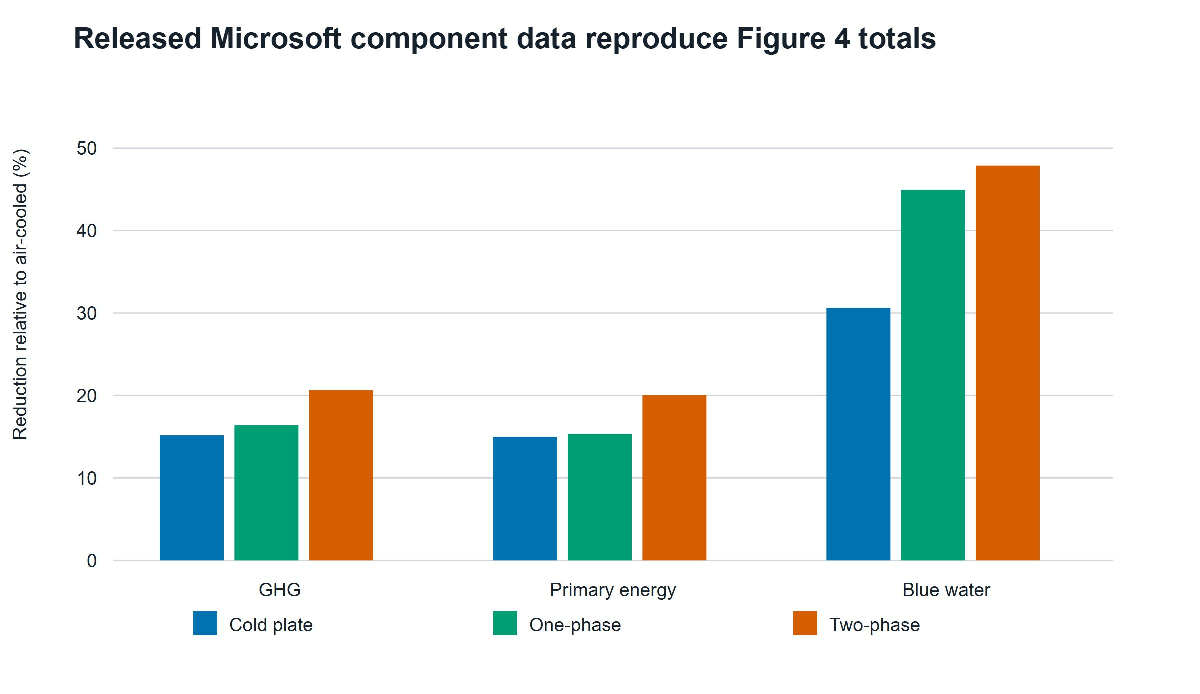
\includegraphics[width=0.98\linewidth]{figures/figure1_microsoft_grid_reductions.pdf}
\caption{Relative reductions versus air cooling obtained by summing the released Microsoft/WSP normalized contributions. All 24 totals were reconciled at workbook precision. This figure reproduces released arithmetic; it does not validate proprietary inventories or field performance.}
\label{fig:figure1-microsoft-grid-reductions}
\end{figure}

\subsection{Historical grid decarbonization is robust to the eGRID GWP update}
The common-basis U.S. generation factor declined from 517.731 kg CO2e/MWh in 2012 to 349.667 kg CO2e/MWh in 2023, a 32.462\% reduction. The trajectory was not monotonic: the factor rose from 373.097 in 2020 to 388.699 in 2021 before declining. Reconstructing every year with AR5 GWP100 changed the provider-published national rate by no more than 0.248 kg CO2e/MWh, in 2012. Thus, the long-run decline is not an artifact of switching from SAR to AR4 and AR5. The direct CO2-only rate was 348.000 kg/MWh in 2023, confirming that CO2 dominates the eGRID total.

The 50-state-plus-DC reconstruction matched the official national total through 2018. From 2019 onward it was 0.32-0.43\% lower because the panel covered 99.55-99.58\% of the provider U.S. generation after excluding Puerto Rico. This scope audit supports use of the provider U.S. aggregate for the national series.

Applying the fixed released foreground model reduced the national air-cooled screen from 36.230 to 25.613 kg CO2e/Vcore-year and the two-phase screen from 28.746 to 20.333. The absolute two-phase-versus-air difference contracted 29.45\%, from 7.484 to 5.280 kg CO2e/Vcore-year, while the air-cooled embodied share rose from 9.69\% to 13.71\%.

\begin{figure}[!htbp]
\centering
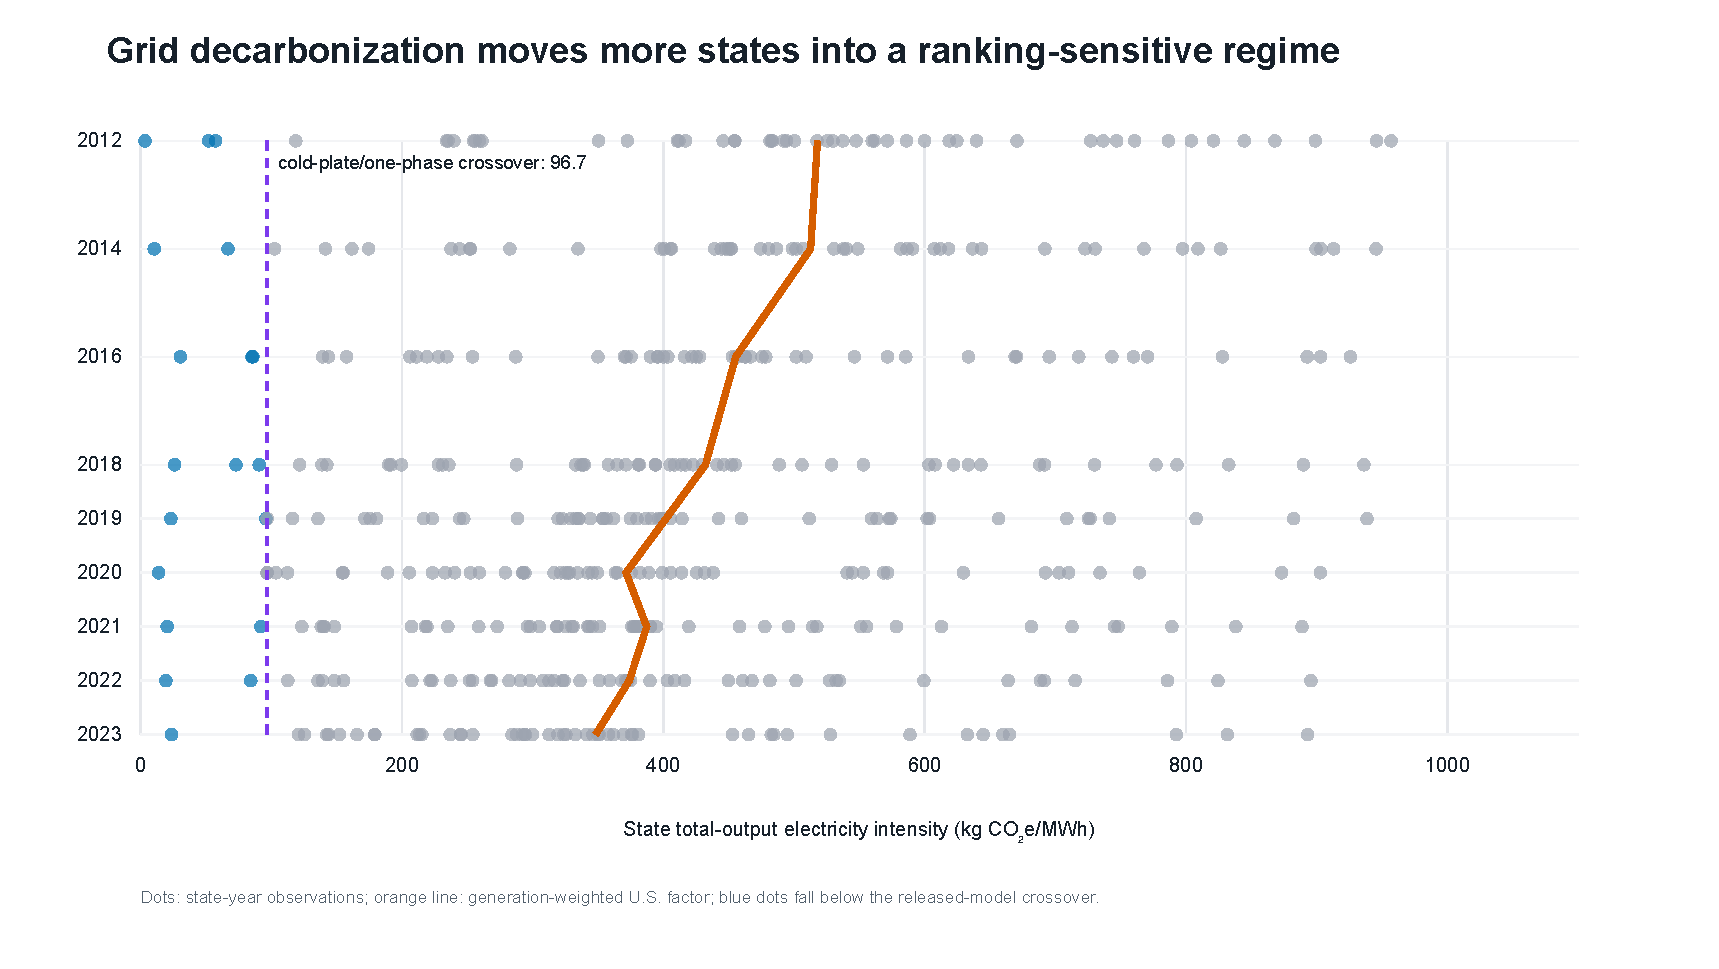
\includegraphics[width=0.98\linewidth]{figures/figure6_historical_grid_transition.pdf}
\caption{Harmonized AR5-GWP100 eGRID state/DC generation rates for nine releases. Orange denotes the provider U.S. aggregate. Blue points fall below the released-model cold-plate/single-phase crossover. The panel shows generation-rate scenarios, not consumption-based lifecycle electricity or independent state LCAs.}
\label{fig:figure6-historical-grid-transition}
\end{figure}

\subsection{The local crossover is more sensitive to boundary than to historical GWP convention}
The cold-plate/single-phase crossover calculated from the two released endpoints was 96.704 kg CO2e/MWh. At unadjusted 2023 eGRID rates, Vermont (23.695 kg CO2e/MWh) was the only state below the crossover; the other 50 state/DC records favored single-phase over cold plate. Arkansas (452.873 kg CO2e/MWh) was well above it. Two-phase remained the deterministic first-ranked architecture in all 51 records.

However, the transformation was not interpolation for much of the panel. Across 459 state-years, 322 rates were between the released anchors, one below the wind anchor, and 136 above the grid anchor. Thus 137 records, or 29.85\%, required extrapolation. In 2023, 9 of 51 rates (17.65\%) exceeded the released grid anchor.

The boundary allowance revealed a sharper limitation. The Vermont cold-plate/single-phase result persisted with 25 and 50 kg CO2e/MWh added to the direct generation rate, but disappeared at 75 and 100 kg CO2e/MWh. The analytical clearance was 96.704-23.695 = 73.009 kg CO2e/MWh; 75 kg CO2e/MWh is therefore only the first point in the declared 25-unit grid above the exact threshold, not an estimate of upstream emissions. Two-phase remained first in 51/51 states across all five allowance levels. This does not estimate the missing upstream inventory. It shows that the headline ``one state below the crossover'' is conditional on treating methodologically different electricity results as a common numerical index.

\subsection{Foreground variation and dependence weaken a deterministic first rank}
Figure 4 consolidates the extrapolation, boundary, zero-correlation all-block stress, and functional-unit diagnostics. Under the 2023 U.S. generation context, two-phase first-rank frequency was 99.19\% in the narrow envelope, 76.17\% in the screening envelope, and 55.05\% in the wide envelope. Cold plate, single-phase, and air cooling had wide-envelope first-rank frequencies of 19.15\%, 25.47\%, and 0.34\%, respectively.

Sensitivity was greater at the lowest-carbon state. Two-phase first-rank frequency was 63.03\%, 42.72\%, and 32.43\% in the narrow, screening, and wide envelopes. Even a narrow perturbation matters when use-phase burdens contract and the alternatives are close. These values are not technology-success probabilities. They quantify how frequently a ranking survives a specified assumption design.

The deterministic functional-unit diagnostic reached the same conclusion from another direction. Across 2023 states, the median adverse correction to two-phase impact per equivalent useful computation required to equal the runner-up was 5.503\%; the range was 5.236-6.042\%. Across all 459 state-years, the median was 5.436\%. A useful-computation correction of this magnitude is small enough that server count, throughput, throttling, reliability, and lifetime must be measured rather than assumed for a decision-grade claim.

\begin{figure}[!htbp]
\centering
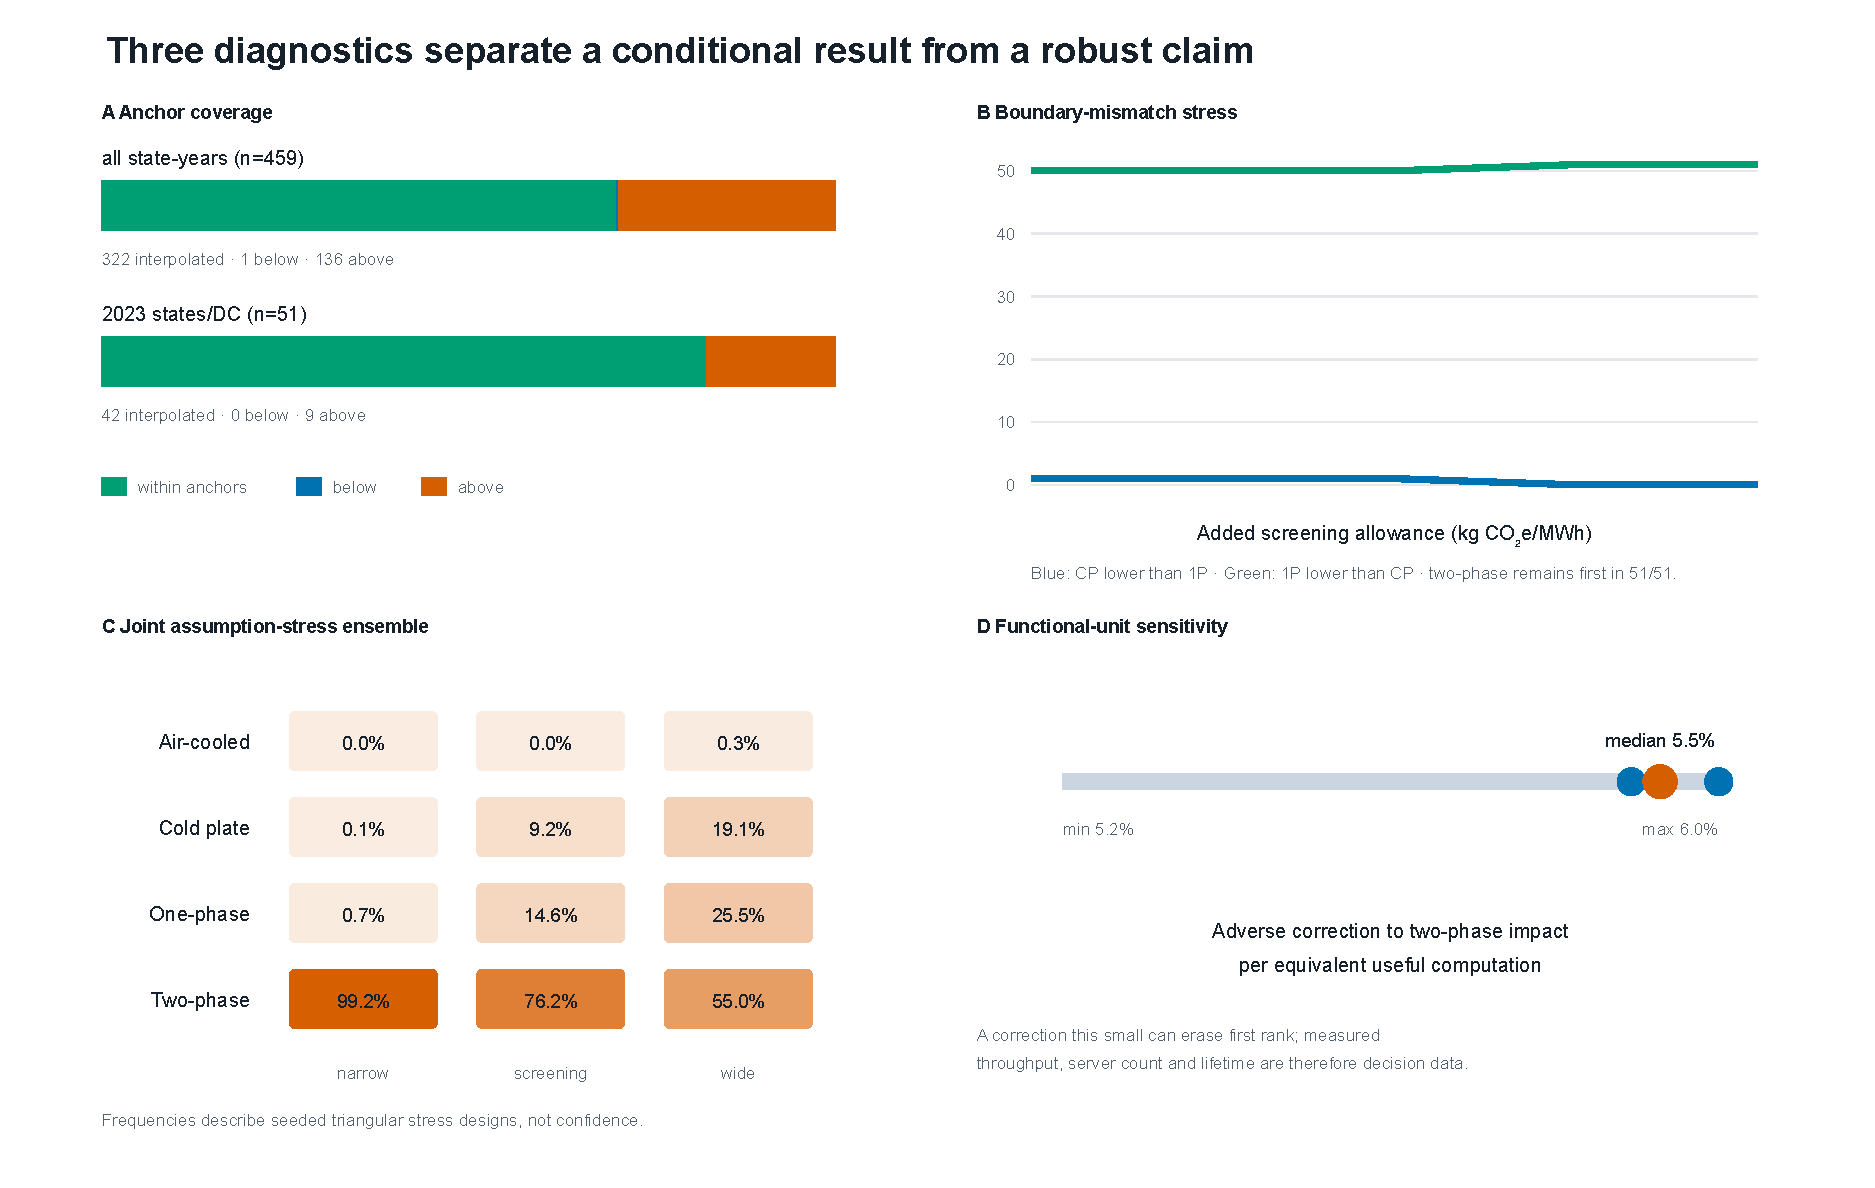
\includegraphics[width=0.98\linewidth]{figures/figure8_scope_uncertainty.pdf}
\caption{Robustness diagnostics. (A) Anchor interpolation and extrapolation counts. (B) Cold-plate/single-phase order under a transparent electricity-boundary allowance. (C) U.S. first-rank frequencies under declared joint stress envelopes. (D) two-phase impact-per-service correction required to erase first rank. Stress frequencies are not confidence levels.}
\label{fig:figure8-scope-uncertainty}
\end{figure}

The block-and-dependence analysis explains why those frequencies change (Figure 5). Grid-rate variation alone never displaced two-phase in any tested U.S. design. In the screening envelope with independent technology-specific errors, two-phase retained first rank in 98.29\% of use-only, 86.75\% of embodied-only, and 96.00\% of service-only draws; with all blocks active the frequency was 76.17\%. The wide-envelope counterparts were 79.52\%, 63.36\%, 73.90\%, and 55.05\%. Embodied variation was therefore the largest one-block source of rank loss under the declared marginal widths.

Dependence was equally important. In the wide all-block design, the U.S. two-phase first-rank frequency increased from 55.05\% at zero latent correlation to 64.50\% at 0.5 and 100\% when technology-specific errors were fully common-mode. The last case does not prove robustness; it shows that common errors preserve relative ordering while independent architecture errors erode it. A rank frequency without a defensible correlation model is therefore under-specified even when every marginal range is disclosed.

The nested convergence check separated Monte Carlo noise from model-form sensitivity. For the three U.S. envelopes, the 20,000-draw frequencies differed from the 80,000-draw results by 0.06, 0.06, and 0.11 percentage points; the 80,000-draw numerical standard errors were 0.031, 0.151, and 0.176 percentage points. Across both locations and all envelopes, the largest 20,000-to-80,000 difference was 0.709 percentage points, for the low-carbon wide case. These differences are small relative to the 44.14-percentage-point change between the U.S. narrow and wide designs and the 44.95-percentage-point change between zero-correlation and common-mode U.S. wide designs. Sampling noise therefore does not explain the central sensitivity result.

\begin{figure}[!htbp]
\centering
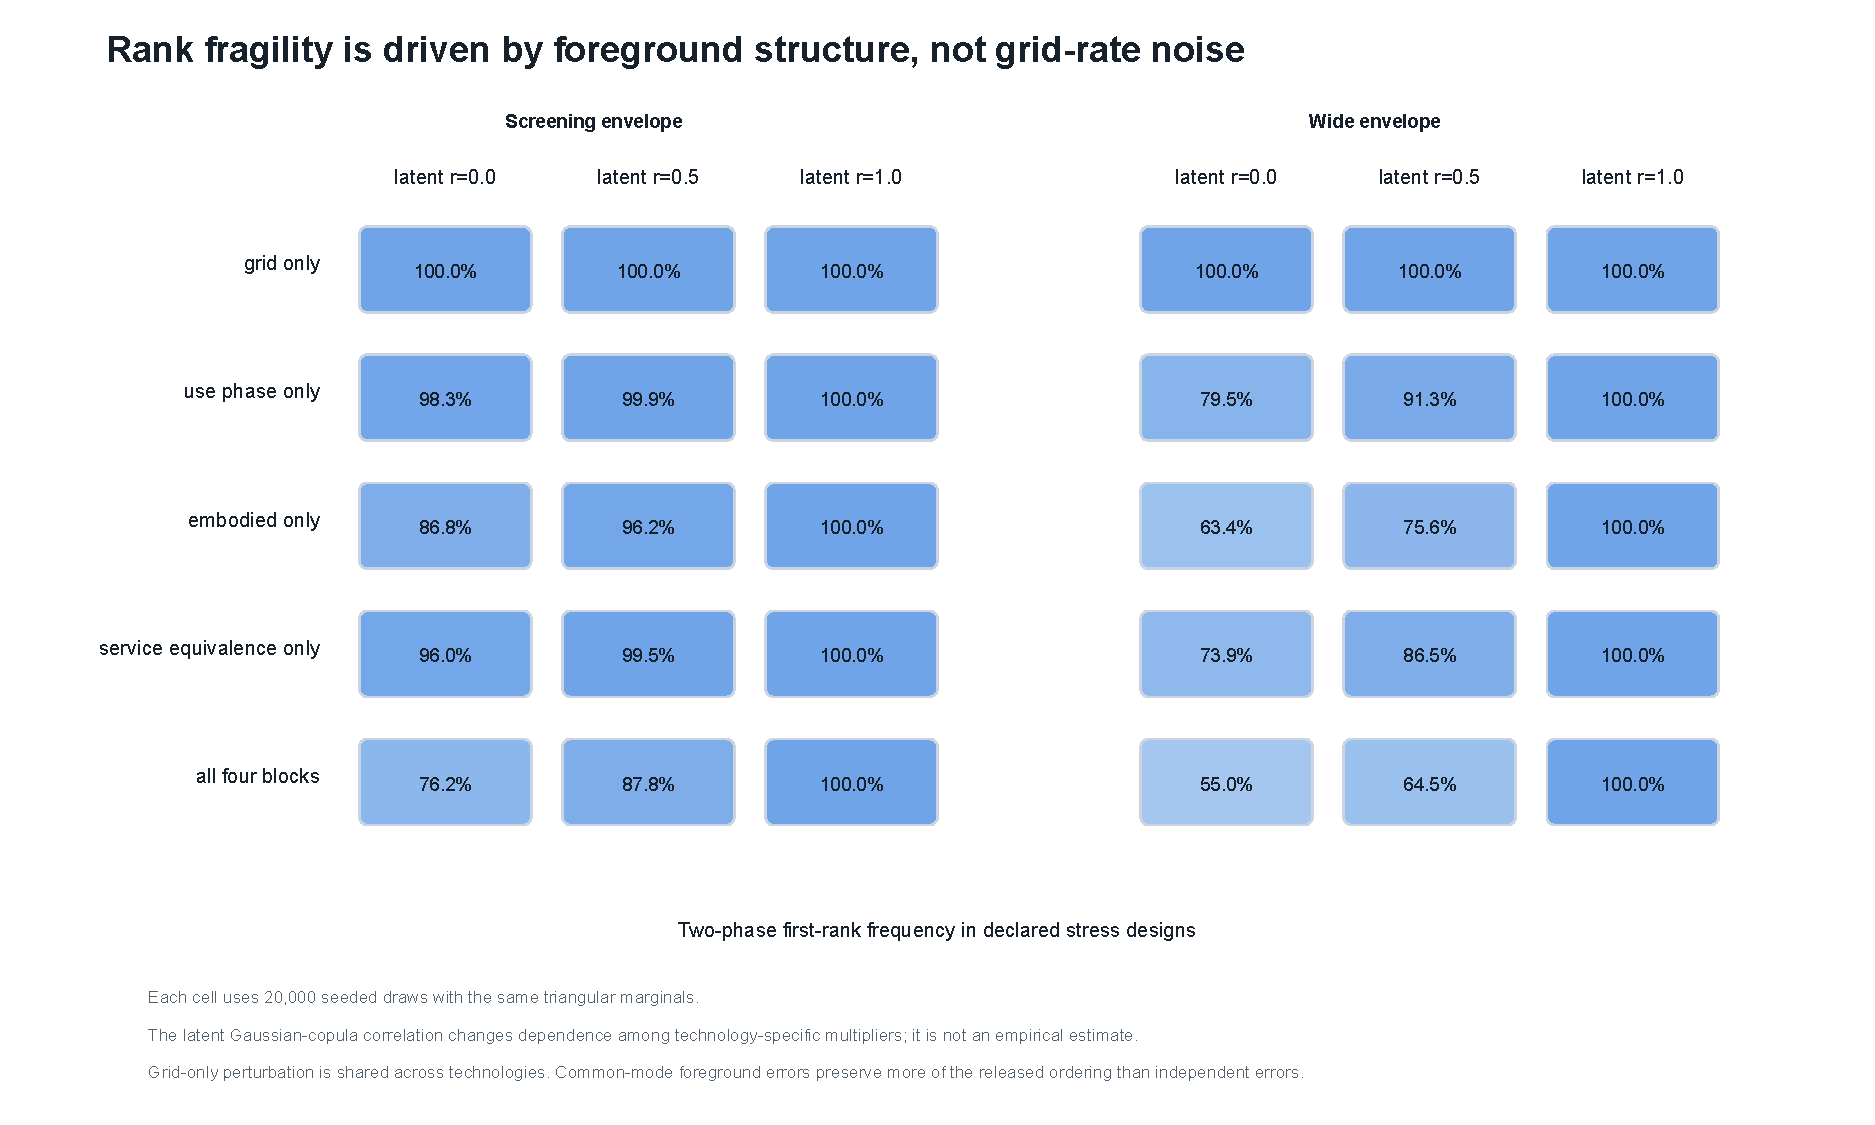
\includegraphics[width=0.98\linewidth]{figures/figure9_stress_structure.pdf}
\caption{Assumption-block and dependence diagnostic for the 2023 U.S. generation context. Cells report two-phase first-rank frequency under declared screening and wide triangular marginals. Grid-only variation is shared. Technology-specific use, embodied, and service multipliers use a Gaussian copula with declared latent correlation. These are sensitivity designs, not empirical probabilities.}
\label{fig:figure9-stress-structure}
\end{figure}

\subsection{Server and construction data reveal leverage but not architecture totals}
The 48 Boavizta server records spanned 465-2,503 kg CO2e/server for manufacturing, a 5.38-fold range. Annualized values spanned 116-626 kg CO2e/server-year. Commonly scaling the released server-related contributions across the empirical 0.38-2.06-fold annualized envelope did not change the deterministic two-phase first rank. That result is a structural stress only: it does not model architecture-specific server count, configuration, throughput, or lifetime.

The selected ÖKOBAUDAT high-scrap electric-arc-furnace galvanized steel record had 59.9\% lower A1-A3 GHG, 47.9\% lower nonrenewable primary energy, and 52.0\% lower freshwater use per kilogram than the selected low-scrap blast-furnace-route record. The selected CEM III cement record had 49.8\% lower GHG, 12.1\% lower nonrenewable primary energy, and 23.5\% lower freshwater use than CEM II/A. These are procurement levers, not data-center reductions. Their facility effect remains unknown until each architecture has a reviewed bill of quantities.

\subsection{Data-priority rank is useful but not invariant}
Under the base contribution-times-weakness index, use phase was the highest priority, followed by storage, networking, and compute-server evidence. Across the nine alternative exponent combinations, use phase ranked first in eight and in the top three in eight. Networking ranked first once; storage was in the top three in all nine; compute was in the top three in four. The rank of use phase ranged from first to fourth.

This sensitivity changes the interpretation of the pedigree result. It supports a near-term measurement sequence---hourly IT and cooling electricity, then server inventories and functional performance---but not a unique value of information. A formal acquisition decision requires empirical parameter distributions, correlations, measurement cost, and the loss associated with a wrong architecture choice \cite{ref30}.

\subsection{Software consistency and practitioner outputs}
With the local evidence archive present, all 49 tests pass. They cover calculation, interoperability, reliability, public-data parsing, practitioner workflow, research analysis, GUI/API parity, endpoint reproduction, eGRID harmonization, extrapolation counts, boundary stress, and functional-unit sensitivity, stress-design determinism, and provenance-integrity checks. In a clone-only clean environment, 41 tests pass and 8 paper-reconstruction tests are skipped explicitly because they require locally held provider files; no dummy data replace those files. The clean install also completed example export, scenario analysis, and practitioner-report generation.

A practitioner supplies IT capacity, utilization, PUE, facility lifetime, onsite water, location- and market-based electricity factors, optional equipment/fluid inventories, and a citable source record. The package returns annual and per-IT-MWh impacts, contribution breakdowns, evidence classification, warnings or blockers, a scenario digest, model version, and the next-data list. Advanced users can add hourly performance maps, replacement and reliability, and openLCA/Brightway inventories. Software consistency does not validate user inputs or make a screening result decision-grade.

\section{Discussion}
\subsection{A cooling ranking should be a decision surface, not a league table}
The released model produces a clear deterministic ranking at its U.S. grid endpoint, and two-phase remains first in every unperturbed state-year screen. If the analysis ended there, the natural conclusion would be that the ranking is broadly transferable. The robustness diagnostics show why that conclusion is too strong.

Cold plate and single-phase cross because their electricity-dependent slopes and non-use-phase intercepts differ. The 96.7 kg CO2e/MWh crossover is a useful engineering result: it identifies where a small operational advantage changes the lifecycle order. It is not a site recommendation because eGRID does not replace the released GaBi electricity process. Similarly, two-phase has a 5-6\% deterministic margin in impact per equivalent service, but its first-rank frequency falls sharply once use, embodied, grid, and service assumptions vary together. A decision surface should therefore report at least the base order, crossover, anchor coverage, boundary sensitivity, functional-unit sensitivity, and evidence class.

\subsection{Characterization harmonization solves a smaller problem than boundary alignment}
Reconstructing the nine eGRID releases to AR5 GWP100 was necessary and reproducible. It also demonstrated that the historical GWP changes have a small numerical effect because power-sector CO2 dominates CH4 and N2O. The 32.46\% national decline is robust to this methodological change.

The boundary mismatch is qualitatively different. eGRID total-output rates omit upstream fuel supply, infrastructure, imports and transmission, while the GaBi anchors are lifecycle results. The two also use GWP100 and GTP100, respectively. No algebra can make them equivalent without a linked inventory and common LCIA method. The exact 73.009 kg CO2e/MWh clearance and the declared 25-unit stress grid are useful because they do not pretend to know the missing value. They show how large an additive boundary term must be to remove the local crossover while leaving its actual physical magnitude unresolved. The deterministic two-phase first rank is less sensitive within this single dimension.

For a decision-grade extension, the correct next step is to replace the intensity index with consumption-based, lifecycle electricity processes calculated under the same LCIA method as the foreground. Location- and market-based cases should be modeled consistently throughout the product system to avoid renewable double counting \cite{ref19,ref20}.

\subsection{Dependence changes the epistemic status of the stress result}
One-at-a-time break-even analysis is easy to interpret but can overstate robustness when inputs co-vary. The stress designs do not provide probability because neither the envelopes nor the copula correlations are fitted. They do yield two negative findings. First, deterministic survival across 459 grid factors does not imply survival under foreground and functional-unit changes; the grid panel explores one dimension repeatedly, not 459 replicates of the cooling technologies. Second, a first-rank frequency is not identified by its marginal ranges alone: the wide all-block value changed from 55.05\% to 100\% when only the dependence design changed from independent to common-mode.

The block decomposition also changes the measurement priority. Under the declared U.S. screening and wide designs, embodied-only variation displaced two-phase more often than use-only, service-only, or grid-only variation. That result does not assign real-world variance to embodied inventories. It shows that architecture-specific quantities, server configurations, service lives, and material inventories deserve the same experimental attention as cooling electricity once operational burdens contract.

This distinction should guide future experiments. Measured distributions are needed for load-dependent fan, pump, coolant-distribution, and heat-rejection power; server throughput and power; fluid loss; component life; and architecture-specific quantities. Correlations matter: a higher coolant temperature may reduce compressor energy while changing chip leakage, performance, and reliability; higher density may reduce building burden per Vcore while increasing local pumping or repair complexity. Empirical joint distributions would convert the present stress frequency into a defensible probability of rank and support expected-value-of-information analysis.

\subsection{Useful computation is the decisive experimental bridge}
Vcore-year is more informative than facility area or rack count, but it is still a proxy. Equivalent useful computation depends on workload, accelerator utilization, memory and network constraints, throttling, overclocking, availability, and quality of service. The median 5.50\% functional-unit threshold is therefore a central result, not merely a limitation. It defines the resolution required of a comparative experiment.

A shared protocol should measure, for every architecture, completed workload or benchmark output; IT and cooling power; inlet and component temperatures; flow and pressure drop; fan, pump, CDU and heat-rejection power; onsite water; failure and maintenance events; and uncertainty/calibration lineage over the same load-weather domain. Server count, configuration, and replacement must be tracked with that performance. A thermal result without useful computation cannot close the LCA functional unit; a product carbon footprint without architecture quantity cannot close the embodied inventory.

\subsection{Decarbonization changes the value of evidence}
The national analysis shows a dual effect. Cleaner generation lowers every electricity-dependent cooling result and contracts the absolute value of operational efficiency, while increasing the fraction supplied by embodied terms. Percentage savings alone hide this transition: the absolute modeled two-phase-versus-air benefit fell 29.45\% between the 2012 and 2023 generation conditions.

This shift explains why the Boavizta and ÖKOBAUDAT datasets matter even though they were not inserted into architecture totals. The 5.38-fold server manufacturing range is larger than many cooling differences, but heterogeneous PCFs cannot be treated as an uncertainty distribution for interchangeable servers. The approximately 50-60\% material-route GHG levers are large per kilogram, but kilograms by architecture are missing. The impactful research contribution is therefore a linked foreground dataset: useful computation, server configuration and lifetime, cooling BOM, material route, and measured operation under one functional unit.

\subsection{Role relative to openLCA, Brightway, and dynamic-LCA tools}
OpenDC-LCA does not compete with openLCA, Brightway, Temporalis, premise, or bw\_timex. Those tools provide process-network calculation, database management, prospective backgrounds, or time-explicit LCA \cite{ref24,ref25,ref26,ref31,ref32}. The contribution here is the cooling-domain contract around them:

\begin{enumerate}
\item a functional-equivalence check tied to useful computation;
\item load-weather cooling performance and bounded annual integration;
\item reliability, replacement, and cooling-fluid representations;
\item explicit separation of lifecycle electricity, direct generation rates,
market instruments, and marginal signals;

\item source and transformation provenance; and
\item a claim gate that prevents exchange success from being mistaken for case
compatibility.

\end{enumerate}

This is why USLCI and GLAD hydrogen archives were exchange-tested but not forced into the results. Backup power is a relevant future application, yet a hydrogen dataset becomes numerical evidence only after technology, electricity source, compression/storage, allocation, geography, and LCIA method are linked to a declared product system.

\subsection{Implications for hyperscale practitioners and the Microsoft study}
The most useful extension of the Microsoft/WSP work is not another static national scenario. It is a jointly governed evidence package that allows the released model to be updated without weakening its functional-unit insight. Four additions would be particularly valuable:

\begin{enumerate}
\item architecture-specific, anonymized bills of quantities and service lives;
\item measured performance surfaces for IT output, server power, facility
parasitics, and onsite water across load and weather;

\item a provider-linked lifecycle electricity model under one LCIA method,
reported alongside location-, market-, and marginal operational signals;

\item empirical uncertainty and correlation information sufficient for rank
probability and value-of-information analysis.

\end{enumerate}

OpenDC-LCA supplies schemas, transformations, tests, and claim boundaries for that collaboration. The present results should interest hyperscale authors because they identify exactly which published conclusions are robust: the released arithmetic and national decarbonization trend. They also identify which are conditional: state-level crossovers, deterministic first rank, and the magnitude of embodied leverage.

\subsection{Limitations and submission-grade evidence needs}
The analysis remains secondary. It does not recreate proprietary background inventories, confidential bills of quantities, the full virtual-core model, or measured hyperscale operation. Equation (8) uses a numerical index across different electricity boundaries and climate metrics. The additive boundary allowance, triangular marginals, and Gaussian-copula dependence cases are diagnostics, not estimates. The convergence check limits numerical sampling error within those designs; it does not reduce epistemic uncertainty in the ranges, dependence structure, or foreground model. State total-output rates represent generation rather than consumption and omit imports, contracts, transmission, hourly dispatch, and marginal effects.

The Boavizta sample mixes products and methods. ÖKOBAUDAT records are German generic A1-A3 factors. The TMY and synthetic performance examples validate software pathways, not technology performance. The USGS file provides watershed geometry rather than water consumption or AWARE characterization. Reliability models omit dependent failures, repair queues, redundancy and maintenance logistics unless the user supplies them. A coauthor methodology review is not an independent critical review.

Before a public decision-grade comparative assertion, the study needs reviewed primary performance and useful-computation data, architecture bills of quantities, lifecycle-consistent electricity inventories, water-scarcity characterization, empirically supported uncertainty/correlation, and an external critical reviewer. These needs are recorded in the repository rather than obscured by additional proxy scenarios.

\section{Conclusions}
OpenDC-LCA treats data-center cooling LCA as an evidence-bounded decision problem. It reconciled 24 released Microsoft/WSP totals, reconstructed nine eGRID releases to a common AR5 GWP100 basis, and quantified extrapolation, electricity-boundary, functional-unit, assumption-block, and dependence sensitivity.

Four findings follow. First, the U.S. generation-rate decline of 32.46\% from 2012 to 2023 is robust to historical eGRID GWP changes; the largest common-basis correction was only 0.248 kg CO2e/MWh. Second, local cooling rankings are less robust: 29.85\% of state-year rates fall outside the released anchors, and the sole 2023 cold-plate/single-phase reversal has an exact 73.009 kg CO2e/MWh additive boundary clearance. Third, deterministic first rank is not stress robustness. Two-phase ranked first in all 459 unperturbed screens, but its U.S. first-rank frequency fell from 99.19\% to 55.05\% across zero-correlation all-block narrow-to-wide designs, and a median 5.50\% adverse useful-computation correction erased first rank. Fourth, the stress frequency itself depends on structure: in the wide U.S. all-block design it ranged from 55.05\% under independent architecture errors to 100\% under fully common-mode errors, while grid-only variation never displaced two-phase.

The practical implication is straightforward: publish cooling comparisons with their functional unit, electricity boundary, anchor coverage, crossover, stress envelope, and evidence class. As grids decarbonize, useful computation, server manufacturing and lifetime, cooling-system quantities, and material routes become first-order research data. The package makes those requirements executable through open schemas, source lineage, engineering models, interoperability, and machine-readable claim gates. The next advance must come from linked primary measurements and inventories, not more precise interpretation of incompatible secondary factors.

\section{Data and code availability}
OpenDC-LCA version 1.1.0 source code, examples, documentation, tests, derived tables, and manuscript figures are available at \url{https://github.com/UARK-NED3/OpenDC-LCA}. Installable wheel and source archives are available from \url{https://github.com/UARK-NED3/OpenDC-LCA/releases/tag/v1.1.0}. No DOI-bearing archive has yet been minted. The repository commit, analysis metadata, and provider-file checksum manifest identify the current reproducibility state; an immutable archival deposit remains a pre-submission action. Provider-native raw files remain local when redistribution permission has not been established. The Microsoft/Nature archive is available from Zenodo \cite{ref15}; eGRID and NOAA data are available from their public portals \cite{ref36,ref37,ref40}.

\begin{thebibliography}{99}
\bibitem{ref1} Masanet, E., Shehabi, A., Lei, N., Smith, S. \& Koomey, J. Recalibrating global data center energy-use estimates. \textit{Science} \textbf{367}, 984-986 (2020). \url{https://doi.org/10.1126/science.aba3758}
\bibitem{ref2} International Energy Agency. Data centres and data transmission networks. \url{https://www.iea.org/energy-system/buildings/data-centres-and-data-transmission-networks}
\bibitem{ref3} Khalaj, A. H. \& Halgamuge, S. K. A review on efficient thermal management of air- and liquid-cooled data centers. \textit{Applied Energy} \textbf{205}, 1165-1184 (2017). \url{https://doi.org/10.1016/j.apenergy.2017.08.037}
\bibitem{ref4} Alkrush, A. A., Salem, M. S., Abdelrehim, O. \& Hegazi, A. A. Data centers cooling: a critical review of techniques, challenges, and energy saving solutions. \textit{International Journal of Refrigeration} \textbf{160}, 246-262 (2024). \url{https://doi.org/10.1016/j.ijrefrig.2024.02.007}
\bibitem{ref5} Kanbur, B. B., Wu, C., Fan, S. \& Duan, F. Two-phase liquid-immersion data center cooling system: experimental performance and thermoeconomic analysis. \textit{International Journal of Refrigeration} \textbf{118}, 290-301 (2020). \url{https://doi.org/10.1016/j.ijrefrig.2020.05.026}
\bibitem{ref6} Kanbur, B. B., Wu, C., Fan, S. \& Duan, F. System-level experimental investigations of direct immersion cooling data center units with thermodynamic and thermoeconomic assessments. \textit{Energy} \textbf{217}, 119373 (2021). \url{https://doi.org/10.1016/j.energy.2020.119373}
\bibitem{ref7} Huang, Y., Liu, B., Xu, S., Bao, C., Zhong, Y. \& Zhang, C. Experimental study on immersion liquid cooling performance of high-power data center servers. \textit{Energy} \textbf{297}, 131195 (2024). \url{https://doi.org/10.1016/j.energy.2024.131195}
\bibitem{ref8} Wu, X. et al. Investigations on heat dissipation performance and overall characteristics of two-phase liquid immersion cooling systems for data center. \textit{International Journal of Heat and Mass Transfer} \textbf{239}, 126575 (2025). \url{https://doi.org/10.1016/j.ijheatmasstransfer.2024.126575}
\bibitem{ref9} Whitehead, B., Andrews, D., Shah, A. \& Maidment, G. Assessing the environmental impact of data centres. Part 1: background, energy use and metrics. \textit{Building and Environment} \textbf{82}, 151-159 (2014). \url{https://doi.org/10.1016/j.buildenv.2014.08.021}
\bibitem{ref10} Siddik, M. A. B., Shehabi, A. \& Marston, L. The environmental footprint of data centers in the United States. \textit{Environmental Research Letters} \textbf{16}, 064017 (2021). \url{https://doi.org/10.1088/1748-9326/abfba1}
\bibitem{ref11} Ristic, B., Madani, K. \& Makuch, Z. The water footprint of data centers. \textit{Sustainability} \textbf{7}, 11260-11284 (2015). \url{https://doi.org/10.3390/su70811260}
\bibitem{ref12} Isler-Kaya, A. \& Karaosmanoglu, F. Life cycle assessment of a climate-friendly data center cooling device. \textit{Energy and Buildings} \textbf{288}, 113006 (2023). \url{https://doi.org/10.1016/j.enbuild.2023.113006}
\bibitem{ref13} Wenzel, P. M. \& Radgen, P. Extending effectiveness to efficiency: comparing energy and environmental assessment methods for a wet cooling tower. \textit{Journal of Industrial Ecology} \textbf{27}, 693-706 (2023). \url{https://doi.org/10.1111/jiec.13396}
\bibitem{ref14} Alissa, H. et al. Using life cycle assessment to drive innovation for sustainable cool clouds. \textit{Nature} \textbf{641}, 331-338 (2025). \url{https://doi.org/10.1038/s41586-025-08832-3}
\bibitem{ref15} Alissa, H. et al. Data and model archive for ``Using life cycle assessment to drive innovation for sustainable cool clouds.'' Zenodo record 14268168 (2024). \url{https://doi.org/10.5281/zenodo.14268168}
\bibitem{ref16} Zhang, M., Carbajales-Dale, M., Ma, X., Guo, L. \& Fan, C. Cleaner grid or smarter cooling? Environmental impact trade-offs of a data center using the life cycle assessment method. \textit{Cleaner Energy Systems} \textbf{12}, 100223 (2025). \url{https://doi.org/10.1016/j.cles.2025.100223}
\bibitem{ref17} Boyd, S. B., Horvath, A. \& Dornfeld, D. Life-cycle assessment of computational logic produced from 1995 through 2010. \textit{Environmental Science \& Technology} \textbf{47}, 2947-2954 (2013). \url{https://doi.org/10.1021/es303012r}
\bibitem{ref18} Malmodin, J. \& Lundén, D. The energy and carbon footprint of the global ICT and E\&M sectors 2010-2015. \textit{Sustainability} \textbf{10}, 3027 (2018). \url{https://doi.org/10.3390/su10093027}
\bibitem{ref19} Holzapfel, P., Bach, V. \& Finkbeiner, M. Electricity accounting in life cycle assessment: the challenge of double counting. \textit{International Journal of Life Cycle Assessment} \textbf{28}, 771-787 (2023). \url{https://doi.org/10.1007/s11367-023-02158-w}
\bibitem{ref20} Holzapfel, P., Bunsen, J., Schmidt-Sierra, I., Bach, V. \& Finkbeiner, M. Replacing location-based electricity consumption with market-based residual mixes in background data to avoid possible double counting. \textit{International Journal of Life Cycle Assessment} \textbf{29}, 1279-1289 (2024). \url{https://doi.org/10.1007/s11367-024-02294-x}
\bibitem{ref21} Dandres, T., Farrahi Moghaddam, R., Nguyen, K. K., Lemieux, Y., Samson, R. \& Cheriet, M. Consideration of marginal electricity in real-time minimization of distributed data centre emissions. \textit{Journal of Cleaner Production} \textbf{143}, 116-124 (2017). \url{https://doi.org/10.1016/j.jclepro.2016.12.143}
\bibitem{ref22} Sohn, J., Kalbar, P., Goldstein, B. \& Birkved, M. Defining temporally dynamic life cycle assessment: a review. \textit{Integrated Environmental Assessment and Management} \textbf{16}, 314-323 (2020). \url{https://doi.org/10.1002/ieam.4235}
\bibitem{ref23} Beloin-Saint-Pierre, D. et al. Addressing temporal considerations in life cycle assessment. \textit{Science of the Total Environment} \textbf{743}, 140700 (2020). \url{https://doi.org/10.1016/j.scitotenv.2020.140700}
\bibitem{ref24} Cardellini, G., Mutel, C. L., Vial, E. \& Muys, B. Temporalis, a generic method and tool for dynamic life cycle assessment. \textit{Science of the Total Environment} \textbf{645}, 585-595 (2018). \url{https://doi.org/10.1016/j.scitotenv.2018.07.044}
\bibitem{ref25} Müller, A. et al. Time-explicit life cycle assessment: a flexible framework for coherent consideration of temporal dynamics. \textit{International Journal of Life Cycle Assessment} (2025). \url{https://doi.org/10.1007/s11367-025-02539-3}
\bibitem{ref26} Diepers, T., Müller, A. \& Jakobs, A. bw\_timex: a Python package for time-explicit life cycle assessment. \textit{Journal of Open Source Software} \textbf{11}, 9621 (2026). \url{https://doi.org/10.21105/joss.09621}
\bibitem{ref27} Michiels, F. \& Geeraerd, A. How to decide and visualize whether uncertainty or variability is dominating in life cycle assessment results: a systematic review. \textit{Environmental Modelling \& Software} \textbf{133}, 104841 (2020). \url{https://doi.org/10.1016/j.envsoft.2020.104841}
\bibitem{ref28} Lloyd, S. M. \& Ries, R. Characterizing, propagating, and analyzing uncertainty in life-cycle assessment: a survey of quantitative approaches. \textit{Journal of Industrial Ecology} \textbf{11}, 161-179 (2007). \url{https://doi.org/10.1162/jiec.2007.1136}
\bibitem{ref29} Edelen, A. \& Ingwersen, W. Guidance on Data Quality Assessment for Life Cycle Inventory Data. U.S. EPA, EPA/600/R-16/096 (2016). \url{https://cfpub.epa.gov/si/si_public_record_report.cfm?Lab=NRMRL&dirEntryId=321834}
\bibitem{ref30} Marchese, D. C., Bates, M. E., Keisler, J. M., Alcaraz, M. L., Linkov, I. \& Olivetti, E. A. Value of information analysis for life cycle assessment: uncertain emissions in green manufacturing of electronic tablets. \textit{Journal of Cleaner Production} \textbf{197}, 1540-1545 (2018). \url{https://doi.org/10.1016/j.jclepro.2018.06.113}
\bibitem{ref31} International Organization for Standardization. ISO 14040:2006, Environmental management - Life cycle assessment - Principles and framework; and ISO 14044:2006, Environmental management - Life cycle assessment - Requirements and guidelines. \url{https://www.iso.org/committee/54854/x/catalogue/;} \url{https://www.iso.org/standard/38498.html}
\bibitem{ref32} International Organization for Standardization. ISO 14071:2024, Environmental management - Life cycle assessment - Critical review processes and reviewer competencies (2024). \url{https://www.iso.org/standard/82464.html}
\bibitem{ref33} GreenDelta. openLCA: open source life cycle assessment software. \url{https://www.openlca.org/}
\bibitem{ref34} Mutel, C. Brightway: an open source framework for life cycle assessment. \textit{Journal of Open Source Software} \textbf{2}, 236 (2017). \url{https://doi.org/10.21105/joss.00236}
\bibitem{ref35} UARK-NED3. OpenDC-LCA version 1.1.0. \url{https://github.com/UARK-NED3/OpenDC-LCA}
\bibitem{ref36} U.S. Environmental Protection Agency. Emissions \& Generation Resource Integrated Database (eGRID), detailed data. \url{https://www.epa.gov/egrid/detailed-data}
\bibitem{ref37} U.S. Environmental Protection Agency. Frequent questions about eGRID: global warming potentials and methodology changes. \url{https://www.epa.gov/egrid/frequent-questions-about-egrid}
\bibitem{ref38} Boavizta. BoaviztAPI data repository. \url{https://github.com/Boavizta/boaviztapi}
\bibitem{ref39} Bundesinstitut für Bau-, Stadt- und Raumforschung. ÖKOBAUDAT 2024-II. \url{https://www.oekobaudat.de/}
\bibitem{ref40} National Centers for Environmental Information. Typical Meteorological Year data. \url{https://www.ncei.noaa.gov/access/typical-meteorological-year/}
\bibitem{ref41} National Renewable Energy Laboratory. U.S. Life Cycle Inventory Database, version 1.2026-06.0. Federal LCA Commons. \url{https://www.lcacommons.gov/}
\bibitem{ref42} United Nations Environment Programme. Global LCA Data Access network. \url{https://www.globallcadataaccess.org/}
\bibitem{ref43} U.S. Geological Survey. Watershed Boundary Dataset. \url{https://www.usgs.gov/national-hydrography/watershed-boundary-dataset}
\end{thebibliography}
\end{document}
